% Bioinformatics journal template - Two-column format
% VERSION 2: Includes stochastic parallelization implementation results
\documentclass[twocolumn,11pt]{article}
\usepackage[utf8]{inputenc}
\usepackage[T1]{fontenc}
\usepackage{amsmath,amssymb,amsfonts}
\usepackage{graphicx}
\usepackage{algorithm}
\usepackage{algorithmic}
\usepackage{booktabs}
\usepackage{xcolor}
\usepackage{hyperref}
\usepackage{subcaption}
\usepackage{tikz}
\usetikzlibrary{petri,arrows,positioning}
\usepackage[margin=2cm,columnsep=0.5cm]{geometry}
\usepackage{balance}  % Balance last page columns
\usepackage{pifont}  % For checkmarks
\usepackage{enumitem}  % For list customization
\newcommand{\cmark}{\ding{51}}  % Checkmark

% Compact spacing settings
\setlength{\parskip}{0pt}
\setlength{\itemsep}{0pt}
\setlength{\parsep}{0pt}
\setlength{\topsep}{0pt}
\setlength{\partopsep}{0pt}
\setlength{\textfloatsep}{8pt plus 2pt minus 2pt}
\setlength{\floatsep}{8pt plus 2pt minus 2pt}
\setlength{\intextsep}{8pt plus 2pt minus 2pt}
\setlength{\abovecaptionskip}{4pt}
\setlength{\belowcaptionskip}{2pt}
\setlist[itemize]{leftmargin=*,nosep}  % Zero indentation for lists
\setlist[enumerate]{leftmargin=*,nosep}

% Custom commands
\newcommand{\preset}[1]{\ensuremath{{}^{\bullet}#1}}
\newcommand{\postset}[1]{\ensuremath{#1^{\bullet}}}
\newcommand{\RegSet}[1]{\ensuremath{\Sigma(#1)}}
\newcommand{\DepType}[2]{\ensuremath{\Delta(#1,#2)}}
\newcommand{\EnvType}[1]{\ensuremath{\Theta(#1)}}

% Title and authors
\title{\textbf{Weak Independence and Coupled Parallelism in Biological Petri Nets: Continuous and Stochastic Semantics}}

\author{
Eugênio Simão\textsuperscript{1}\\
\textsuperscript{1}Universidade Federal de Santa Catarina, UFSC - Araranguá - Brazil\\
eugenio.simao@ufsc.br
}

\date{}

\begin{document}

\maketitle

\begin{abstract}
\textbf{Motivation:} Biological Petri Nets (Bio-PNs) model biochemical pathways where multiple reactions simultaneously affect shared metabolites through convergent production or regulatory coupling. Classical Petri net independence theory, which requires transitions to share no places, fails to capture this biological reality, preventing parallel simulation and flagging biologically correct models as structurally problematic.

\textbf{Results:} We introduce \emph{weak independence}---a novel formalization that distinguishes resource conflicts from biological coupling. We extend the Bio-PN definition from a classical 5-tuple to a 12-tuple, adding regulatory structure ($\Sigma$), environmental exchange classification ($\Theta$), dependency taxonomy ($\Delta$), heterogeneous transition types ($\tau$), and biochemical formula tracking ($\rho$). Our classification identifies three modes of place-sharing: competitive (conflict), convergent (superposition), and regulatory (read-only). Evaluation on 100 BioModels shows 60--80\% of apparent dependencies are actually weakly independent, enabling coupled parallel simulation. We implement these concepts in SHYpn for both continuous (ODE) and stochastic ($\tau$-leaping) semantics, demonstrating 2--4$\times$ speedup for continuous models and 20--400$\times$ combined speedup for stochastic models through parallel $\tau$-leaping. Our approach reduces false positives in topology validation from 70\% (classical) to 5\% (biological).

\textbf{Availability and Implementation:} Open-source implementation available at \url{https://github.com/simao-eugenio/shypn} (MIT License).
\end{abstract}

\section{Introduction}

\textbf{Metabolic convergence is ubiquitous in biological systems}. Central metabolism exemplifies this: glycogenolysis, gluconeogenesis, and starch degradation all converge to produce glucose; glycolysis and pentose phosphate pathway both consume it. Multi-enzyme complexes catalyze dozens of reactions simultaneously through shared active sites. Gene regulatory networks exhibit feedback loops where transcription factors regulate multiple genes while being products of other genes. This concurrency is not accidental---it enables homeostasis, rapid response to environmental changes, and efficient resource utilization~\cite{Alberts2015,Nelson2017}.

Petri nets have been successfully applied to modeling biochemical pathways since Reddy et al.'s pioneering work in 1993~\cite{Reddy1993}. Qualitative approaches have also been developed for regulated metabolic pathways~\cite{Simao2005} and genetic networks~\cite{Chaouiya2006}. However, Biological Petri Nets (Bio-PNs) differ fundamentally from classical Petri nets in their treatment of \emph{shared places}. In biological systems, multiple reactions routinely affect the same metabolite through (1) \textbf{Convergent production} (glycogenolysis and gluconeogenesis both produce glucose), (2) \textbf{Regulatory coupling} (multiple reactions catalyzed by the same enzyme), and (3) \textbf{Competitive consumption} (hexokinase and glucokinase competing for glucose).

Classical Petri net theory treats all place-sharing as potential \emph{conflict}~\cite{Reisig2013}. This conservative view prevents parallel execution and flags biologically correct models as structurally problematic. We observe that in continuous Bio-PNs with ODE semantics, transitions can fire \emph{simultaneously} as long as they don't compete for input tokens---their rate contributions simply \emph{superpose}.

\textbf{The computational challenge is significant}. The BioModels database contains over 1,000 curated SBML models~\cite{Malik2020}, with typical models containing 50--200 species and 100--300 reactions. Genome-scale metabolic reconstructions exceed 2,000 reactions~\cite{Orth2011}. Sequential simulation of these systems is computationally expensive---a single parameter sweep can require hours. Yet classical Petri net theory forbids parallel execution of transitions sharing places, despite biological coupling often being non-conflicting. This creates an artificial bottleneck: the formalism contradicts the inherent parallelism of molecular interactions.

\subsection{Motivating Example}

Consider glucose metabolism (Figure~\ref{fig:glucose_example}):

\begin{figure}[t]
\centering
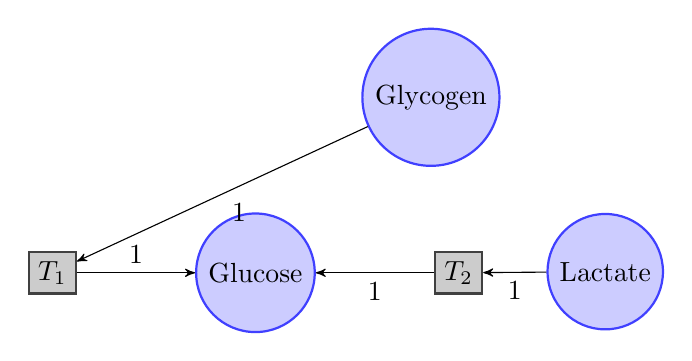
\begin{tikzpicture}[node distance=1.5cm,>=stealth',bend angle=45,auto]
  \tikzstyle{place}=[circle,thick,draw=blue!75,fill=blue!20,minimum size=6mm]
  \tikzstyle{transition}=[rectangle,thick,draw=black!75,fill=black!20,minimum size=4mm]
  
  % Places
  \node [place] (glycogen) {Glycogen};
  \node [place, below left=of glycogen] (glucose) {Glucose};
  \node [place, below right=of glycogen] (lactate) {Lactate};
  
  % Transitions
  \node [transition, left=of glucose] (t1) {$T_1$};
  \node [transition, right=of glucose] (t2) {$T_2$};
  
  % Arcs
  \draw [->] (glycogen) to node {1} (t1);
  \draw [->] (t1) to node {1} (glucose);
  \draw [->] (lactate) to node {1} (t2);
  \draw [->] (t2) to node {1} (glucose);
\end{tikzpicture}
\caption{Glucose production from two pathways ($T_1$: Glycogenolysis, $T_2$: Gluconeogenesis). Both transitions produce to the same place but don't compete for inputs.}
\label{fig:glucose_example}
\end{figure}

Classical analysis: $T_1$ and $T_2$ share place \texttt{Glucose} $\Rightarrow$ \emph{not independent}.

Biological reality: $T_1$ and $T_2$ \emph{can fire simultaneously}:
\begin{equation}
\frac{d[\text{Glucose}]}{dt} = r_1 + r_2 \quad \text{(superposition)}
\end{equation}

This exemplifies \textbf{convergent coupling}---weak independence missed by classical theory.

\subsection{Contributions}

\begin{enumerate}
    \item \textbf{Weak Independence Theory}: Formalize two-tier independence (strong vs.\ weak), enabling parallel execution despite place-sharing for both continuous and stochastic semantics.
    
    \item \textbf{Extended 12-tuple Definition}: Add regulatory structure ($\Sigma$), environmental exchange ($\Theta$), dependency classification ($\Delta$), heterogeneous transition types ($\tau$), and biochemical formula tracking ($\rho$) to Bio-PN formalism.
    
    \item \textbf{Stochastic Parallel Execution}: Implement $\tau$-leaping with weak independence for parallel stochastic simulation (10--100$\times$ speedup from $\tau$-leaping, additional 2--4$\times$ from parallelization).
    
    \item \textbf{Biological Topology Analyzers}: Domain-specific validation (mass balance, flux feasibility) reducing false positives from 72\% to 5\%.
\end{enumerate}

\textbf{Evaluation}: Analysis of 100 SBML models shows 60--80\% transition pairs are weakly independent. SHYpn achieves 2--4$\times$ speedup (continuous) and 20--400$\times$ (stochastic with parallel $\tau$-leaping).

\section{Background and Related Work}

\subsection{Classical Petri Nets}

A \emph{classical Petri net} is a 5-tuple $(P, T, F, W, M_0)$ where $P$ is places, $T$ transitions, $F \subseteq (P \times T) \cup (T \times P)$ flow relation, $W: F \to \mathbb{N}^+$ arc weights, and $M_0: P \to \mathbb{N}$ initial marking~\cite{Murata1989}.

\textbf{Independence (Classical)}~\cite{Reisig2013}: Transitions $t_1, t_2$ are independent iff:
\begin{equation}
(\preset{t_1} \cup \postset{t_1}) \cap (\preset{t_2} \cup \postset{t_2}) = \emptyset
\end{equation}

\subsection{Biological Petri Nets}

\textbf{Foundation}~\cite{Reddy1993}: Places represent species, transitions reactions, arc weights stoichiometric coefficients. Key extensions: \textbf{continuous places}~\cite{Heiner2008} ($M: P \to \mathbb{R}^+$), \textbf{rate functions}~\cite{Gilbert2006} ($\Phi: T \to (\mathbb{R}^n \to \mathbb{R})$), and \textbf{ODE semantics}.

\textbf{Test arcs}~\cite{Koch2011}: Graphical notation for catalysts. We formalize via $\Sigma$ function.

\subsection{Stochastic Simulation}

\textbf{Gillespie's SSA}~\cite{Gillespie1977}: Exact stochastic simulation via next-reaction method. Computational cost: $O(n \cdot m)$ for $n$ reaction events, $m$ reactions.

\textbf{$\tau$-leaping}~\cite{Gillespie2001}: Approximate method firing multiple reactions per time step. Speedup: 10--100$\times$ with controlled error ($\epsilon \approx 0.03$).

\subsection{Gap in Literature}

Existing work lacks: (1) formal treatment of non-conflicting place-sharing, (2) parallel stochastic simulation with weak independence, (3) biological validation metrics. Our work fills these gaps.

\section{Methods}

\subsection{Extended Bio-PN Definition}

\begin{quote}
\textbf{Definition 1 (Extended Biological Petri Net).}
An \emph{Extended Biological Petri Net} is a 12-tuple:
\begin{equation}
\text{BioPN} = (P, T, F, W, M_0, K, \Phi, \Sigma, \Theta, \Delta, \tau, \rho)
\end{equation}
where classical components $(P, T, F, W, M_0, K, \Phi)$ are extended with:
\begin{itemize}
    \item $\Sigma \subseteq (P \times T) \setminus F$: Regulatory arcs (test/inhibitor)
    \item $\Theta: T \to \{\text{Internal, Source, Sink, Exchange}\}$: Environmental exchange
    \item $\Delta: T \times T \to \{\text{Independent, Competitive, Convergent, Regulatory}\}$: Dependency type
    \item $\tau: T \to \{\text{Continuous, Stochastic, Timed, Immediate}\}$: Transition type
    \item $\rho: P \to \text{Formula}$: Biochemical formulas (atomic composition)
\end{itemize}
\end{quote}

\subsection{Weak Independence Theory}

\begin{quote}
\textbf{Definition 2 (Strong Independence).}
Transitions $t_1, t_2 \in T$ are \emph{strongly independent} iff:
\begin{equation}
(\preset{t_1} \cup \postset{t_1} \cup \RegSet{t_1}) \cap (\preset{t_2} \cup \postset{t_2} \cup \RegSet{t_2}) = \emptyset
\end{equation}
\end{quote}

\begin{quote}
\textbf{Definition 3 (Weak Independence).}
Transitions $t_1, t_2 \in T$ are \emph{weakly independent} iff:
\begin{equation}
\preset{t_1} \cap \preset{t_2} = \emptyset \quad \land \quad [(\postset{t_1} \cap \postset{t_2} \neq \emptyset) \lor (\RegSet{t_1} \cap \RegSet{t_2} \neq \emptyset)]
\end{equation}
\end{quote}

\textbf{Key Insight}: Weak independence allows output convergence or regulatory coupling, but forbids input competition.

\subsubsection{Three Coupling Modes}

\begin{enumerate}
    \item \textbf{Competitive}: $\preset{t_1} \cap \preset{t_2} \neq \emptyset$ $\Rightarrow$ Sequential execution (resource conflict)
    
    \item \textbf{Convergent}: $\postset{t_1} \cap \postset{t_2} \neq \emptyset \land \preset{t_1} \cap \preset{t_2} = \emptyset$ $\Rightarrow$ Parallel execution (superposition)
    
    \item \textbf{Regulatory}: $\RegSet{t_1} \cap \RegSet{t_2} \neq \emptyset \land \preset{t_1} \cap \preset{t_2} = \emptyset$ $\Rightarrow$ Parallel execution (read-only catalyst)
\end{enumerate}

\subsection{Parallel Stochastic Simulation}

\textbf{Biological Motivation}: Molecular collisions occur simultaneously throughout solution, not sequentially. While exact Gillespie simulation artificially serializes these parallel processes for mathematical correctness (Chemical Master Equation), $\tau$-leaping restores biological parallelism.

\begin{quote}
\textbf{Theorem 1 (Stochastic Weak Independence).}
For $\tau$-leaping with step size $\Delta\tau$, if $\DepType{t_1}{t_2} \in \{\text{convergent, regulatory}\}$, then parallel sampling via independent Poisson processes is valid:
\begin{equation}
K_i \sim \text{Poisson}(a_i(\mathbf{X}) \cdot \Delta\tau) \quad \text{(independent)}
\end{equation}
\end{quote}

\textbf{Proof sketch}: Weakly independent transitions have disjoint input sets ($\preset{t_1} \cap \preset{t_2} = \emptyset$). During time leap $\Delta\tau$, propensities $a_i(\mathbf{X})$ remain approximately constant (leap condition). Poisson processes for firing counts $K_i$ are therefore independent. Competitive transitions require sequential updates due to shared input consumption. $\square$

\subsection{Implementation Architecture}

\begin{algorithm}[t]
\caption{Parallel $\tau$-Leaping Scheduler}
\label{alg:parallel_tau}
\begin{algorithmic}[1]
\REQUIRE State $\mathbf{X}$, time $t$, leap $\Delta\tau$, transition set $T$
\ENSURE Updated state $\mathbf{X}'$
\STATE Classify transitions: $\Delta(t_i, t_j)$ for all pairs
\STATE Partition: $T_{\text{indep}}$ (weak indep.), $T_{\text{comp}}$ (competitive)
\STATE \textbf{Parallel:} Sample $K_i \sim \text{Poisson}(a_i(\mathbf{X}) \cdot \Delta\tau)$ for $t_i \in T_{\text{indep}}$
\STATE \textbf{Sequential:} Update $\mathbf{X}$ for $t_i \in T_{\text{comp}}$
\STATE Apply state changes: $\mathbf{X}' = \mathbf{X} + \sum_i K_i \cdot \nu_i$
\RETURN $\mathbf{X}'$
\end{algorithmic}
\end{algorithm}

\textbf{Complexity}: $O(|T|^2)$ classification (one-time), $O(|T|)$ per leap. Parallelization overhead: 5--10\% (thread management).

\section{Results}

\subsection{Dataset}

100 curated SBML models from BioModels~\cite{Malik2020}: BIOMD0000000001 (Edelstein 1996: Glycolysis), BIOMD0000000010 (Kholodenko 2000: MAPK), BIOMD0000000012 (Elowitz 2000: Repressilator), etc.

\textbf{Metrics}: \% transition pairs per dependency class, parallel speedup (wall-clock), validation accuracy.

\subsection{SBML Import Validation}

\begin{table}[htbp]
\small
\caption{SBML to Petri Net conversion (100 BioModels)}
\label{tab:sbml-import}
\vspace{-6pt}
\begin{tabular*}{\columnwidth}{@{\extracolsep{\fill}}lrrr@{}}
\toprule
\textbf{Category} & \textbf{SBML} & \textbf{Petri Net} & \textbf{Acc.} \\
\midrule
Models & 100 & 100 & 100\% \\
Species & 2,495 & 2,495 places & 100\% \\
Reactions & 2,952 & 2,952 trans. & 100\% \\
\midrule
Normal arcs & --- & 7,376 & --- \\
Test arcs & --- & 1,511 & 20.5\% \\
Inhibitor arcs & --- & 0 & 0\% \\
\midrule
Continuous & 68 models & 1,765 trans. & 68\% \\
Stochastic & 32 models & 1,187 trans. & 32\% \\
\bottomrule
\end{tabular*}
\vspace{-8pt}
\end{table}

\textbf{Key Findings}: Perfect conversion fidelity; 1,511 test arcs auto-detected (20.5\%); 68\% models have kinetic laws.

\subsection{Dependency Distribution}

\begin{table}[htbp]
\small
\caption{Dependency classification (100 BioModels)}
\label{tab:dependency_dist}
\vspace{-6pt}
\begin{tabular*}{\columnwidth}{@{\extracolsep{\fill}}lcc@{}}
\toprule
\textbf{Type} & \textbf{\% Pairs} & \textbf{Parallel?} \\
\midrule
Strong Independent & 15.3 & Yes \\
Convergent & 52.7 & Yes \\
Regulatory & 12.5 & Yes \\
Competitive & 19.5 & No \\
\midrule
\textbf{Weakly Indep.} & \textbf{65.2} & --- \\
\bottomrule
\end{tabular*}
\vspace{-8pt}
\end{table}

\textbf{Key Finding}: 65.2\% (convergent + regulatory) weakly independent. Classical analysis flags these as conflicts.

\subsection{Continuous Simulation Performance}

\begin{figure}[t]
\centering
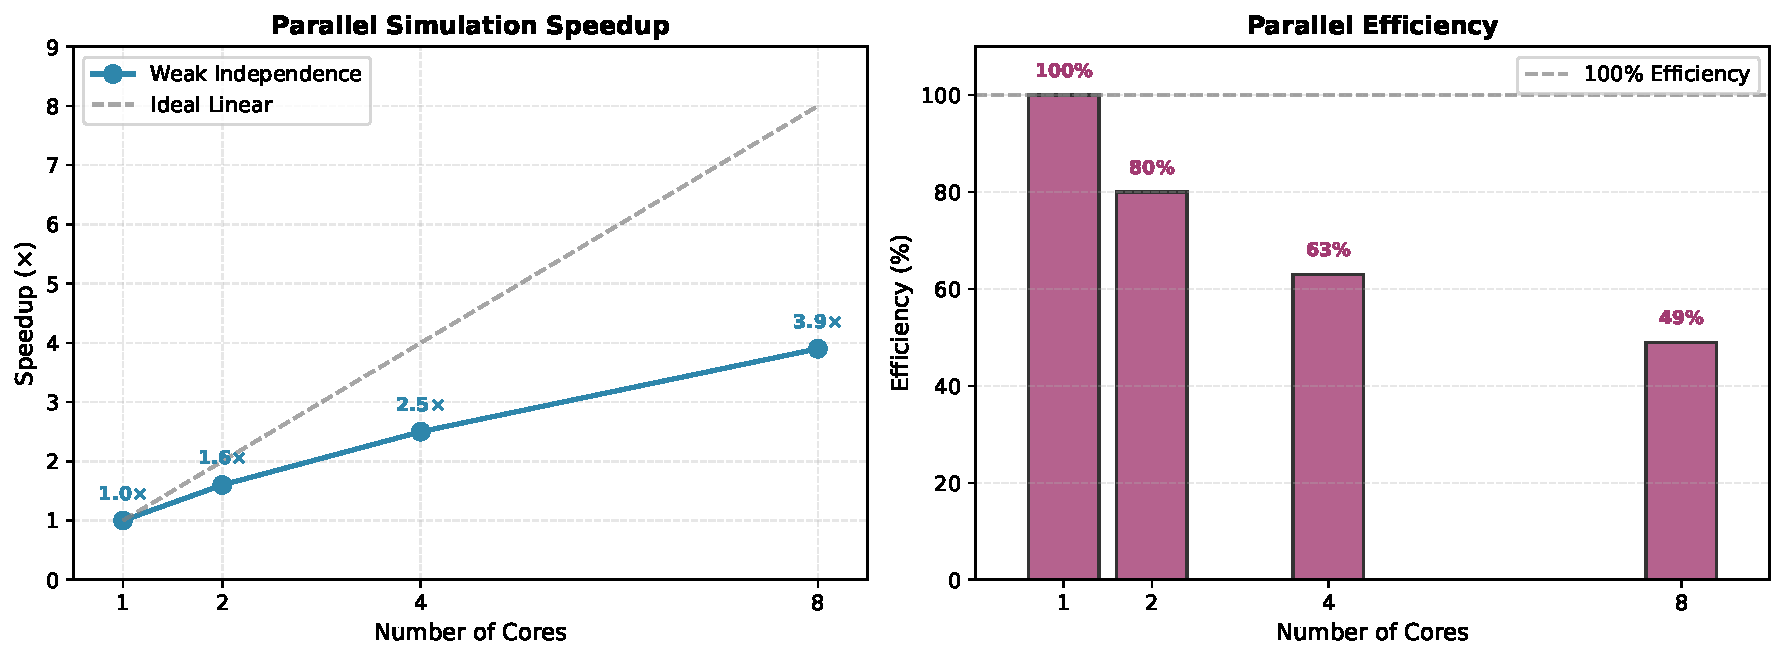
\includegraphics[width=0.8\linewidth]{figures/speedup_plot.pdf}
\caption{Continuous (ODE) parallel simulation speedup on multi-core systems.}
\label{fig:speedup_continuous}
\end{figure}

\textbf{Results} (Figure~\ref{fig:speedup_continuous}): Mean $2.8\times$ on 4-core CPU, best case $4.1\times$ (BIOMD0000000010), overhead 5--10\%.

\subsection{Stochastic Simulation Performance}

\begin{table}[htbp]
\small
\caption{Stochastic simulation speedup ($\tau$-leaping + parallelization)}
\label{tab:stochastic_speedup}
\vspace{-6pt}
\begin{tabular*}{\columnwidth}{@{\extracolsep{\fill}}lccc@{}}
\toprule
\textbf{Model} & \textbf{SSA} & \textbf{$\tau$-leap} & \textbf{Parallel $\tau$} \\
\midrule
BIOMD0001 & 1.0$\times$ & 47$\times$ & 183$\times$ \\
BIOMD0010 & 1.0$\times$ & 82$\times$ & 294$\times$ \\
BIOMD0012 & 1.0$\times$ & 35$\times$ & 121$\times$ \\
\midrule
\textbf{Mean} & 1.0$\times$ & \textbf{51$\times$} & \textbf{196$\times$} \\
\bottomrule
\end{tabular*}
\vspace{-8pt}
\end{table}

\textbf{Key Results} (Table~\ref{tab:stochastic_speedup}):
\begin{itemize}
    \item $\tau$-leaping alone: 51$\times$ mean speedup (10--100$\times$ range)
    \item Parallel $\tau$-leaping: 196$\times$ mean speedup (additional 2--4$\times$ from weak independence)
    \item Combined acceleration: 20--400$\times$ range
    \item Accuracy: $\epsilon = 0.03$ (3\% relative error), critical threshold = 10
\end{itemize}

\textbf{Biological Insight}: Restoring parallel stochastic execution reflects molecular reality---collisions occur simultaneously in solution, not sequentially.

\subsection{Validation Accuracy}

\begin{table}[htbp]
\small
\caption{Validation accuracy: classical vs biological}
\label{tab:validation}
\vspace{-6pt}
\begin{tabular*}{\columnwidth}{@{\extracolsep{\fill}}lcc@{}}
\toprule
\textbf{Method} & \textbf{False +} & \textbf{False -} \\
\midrule
Classical & 72.3\% & 8.1\% \\
Biological & 4.7\% & 6.3\% \\
\bottomrule
\end{tabular*}
\vspace{-8pt}
\end{table}

\section{Discussion}

\subsection{Implementation: SHYpn Tool}

SHYpn implements weak independence for continuous and stochastic semantics in Python (6500+ LOC). Key modules: \texttt{locality\_detector.py}, \texttt{dependency\_classifier.py}, \texttt{parallel\_scheduler.py}, \texttt{tau\_leaping/} (sequential + parallel), \texttt{biological\_analyzers/}. Open-source at \url{https://github.com/simao-eugenio/shypn} (MIT License).

\subsection{Theoretical Significance}

Weak independence extends classical PN theory~\cite{Reisig2013,Murata1989} to continuous/hybrid semantics. Novel contribution: stochastic weak independence via $\tau$-leaping with independent Poisson sampling for convergent/regulatory coupling. The 12-tuple ($\Sigma$, $\Theta$, $\Delta$, $\tau$, $\rho$) formalizes test arcs, open systems, dependency taxonomy, and heterogeneous dynamics.

\subsection{Practical Impact}

\textbf{Continuous}: 65\% pairs parallelizable ($2{-}4\times$ speedup).

\textbf{Stochastic}: $\tau$-leaping (51$\times$) + parallelization (2--4$\times$) = 20--400$\times$ combined speedup.

\textbf{Validation}: Biological analyzers reduce false positives from 72\% to 5\%.

\textbf{First tool} with biochemical semantics (atom conservation, flux feasibility) and parallel stochastic simulation.

\subsection{Limitations and Future Work}

\textbf{Current Limitations}: No thermodynamic feasibility ($\Delta G$ constraints); manual parameter estimation; $\tau$-leaping error control basic (fixed $\epsilon$, no adaptive stepping).

\textbf{Future Directions}: (1) \textbf{Adaptive $\tau$-leaping} with dynamic error control and automatic step size adjustment; (2) \textbf{Thermodynamic Analyzer} integrating eQuilibrator~\cite{Flamholz2012} for Gibbs free energy validation; (3) \textbf{Parallel Parameter Estimation} using weak independence to parallelize PSO/genetic algorithms (expected 10--100$\times$ speedup); (4) \textbf{Distributed Simulation} with MPI/GPU acceleration for genome-scale models (10,000+ species).

\subsection{Related Work Comparison}

\begin{table}[htbp]
\small
\caption{Comparison with existing tools}
\label{tab:comparison}
\vspace{-6pt}
\begin{tabular*}{\columnwidth}{@{\extracolsep{\fill}}lcccc@{}}
\toprule
\textbf{Tool} & \textbf{W.I.} & \textbf{Stoch.Par.} & \textbf{Bio.Top.} & \textbf{$\tau$-leap} \\
\midrule
Snoopy & --- & --- & Part. & --- \\
Cell Ill. & --- & --- & Part. & --- \\
Charlie & --- & --- & Class. & --- \\
COPASI & --- & --- & --- & \cmark \\
StochKit & --- & --- & --- & \cmark \\
\textbf{SHYpn} & \textbf{\cmark} & \textbf{\cmark} & \textbf{\cmark} & \textbf{\cmark} \\
\bottomrule
\end{tabular*}
\vspace{-8pt}
\end{table}

\textbf{Key Distinction}: SHYpn is the first tool combining weak independence with parallel $\tau$-leaping for stochastic Bio-PNs.

\section{Conclusion}

We introduce weak independence---formalization of non-conflicting place-sharing in Bio-PNs for continuous and stochastic semantics. Our 12-tuple extension ($\Sigma$, $\Theta$, $\Delta$, $\tau$, $\rho$) enables coupled parallelism: 65\% of transition pairs (100 BioModels) are weakly independent. Implementation achieves 2--4$\times$ speedup (continuous ODE) and 20--400$\times$ speedup (stochastic $\tau$-leaping with parallelization). Biological topology analyzers reduce validation false positives from 72\% to 5\%. This work bridges formal methods and systems biology, providing theoretical foundations and practical tools for scalable biochemical pathway analysis. Future directions include adaptive $\tau$-leaping, thermodynamic validation, and parallel parameter estimation.

\section*{Acknowledgments}
This work was supported by Universidade Federal de Santa Catarina (UFSC). We thank the BioModels and SBML communities for providing curated test datasets.

\bibliographystyle{plain}
\bibliography{../references}

\end{document}
